\section{Introduction}
\label{sec:intro}

%% Soft robots can do cool things because they are compliant, but are difficult to model and control for the same reason
Soft robots, or robots that incorporate non-rigid materials into their morphology to facilitate compliant interactions with the external world, are being developed for purposes such as manipulating delicate objects, adapting to unstructured environments, and enabling safe interactions with coexisting humans \cite{rus2015design}.
While such robots demonstrate physical capabilities beyond those of traditional rigid-bodied robots, their dynamic behavior is not well-understood \Ram{Can you cite a reference of some kind?}.
The infinite degrees of freedom and highly nonlinear nature of soft materials make it difficult to construct accurate models of soft robots without making significant simplifying assumptions such as constant curvature \cite{rus2015design}, quasi-static \cite{george2018control}, or simplified geometry \cite{bruder2017model} \Ram{you are only referencing a handful of papers despite having an infinite amount of space for references. This is dangerous especially since our competitors are going to review this paper and will expect to be cited..}.
These models only describe behavior well in the subset of robot configurations where all assumptions hold, hence they are limited in applicability \Ram{can you describe with a more concrete example what you mean?}.
% white-box model based on first principles, e.g. a model for a physical process from the Newton equations, but in many cases such models will be overly complex and possibly even impossible to obtain in reasonable time due to the complex nature of many systems and processes

%% Lack of good models poses a problem for control
\Dan{Need to rewrite this paragraph more formally}
This poses a problem for control \Ram{what poses a problem for control. Be specific.}.
When a good model is available, a predictive controller can be built that uses the model to calculate a feedforward term, then feedback can be used to stabilize around that desired point/account for model uncertainty/error (i.e. make up the difference).
However, if a good model is unavailable, feedback must be more heavily relied upon.
Since feedback is reactionary rather than anticipatory, it can be slow to track a set point.
More troublingly, relying heavily on feedback to compensate for an inaccurate model has been shown to reduce the compliance of soft robotic systems \cite{della2017controlling}.
That is, excessive feedback negates the desirable compliance of a soft robot by replacing the its natural dynamics with a slower, stiffer system.
To control soft robots in a manner that reduces dependence on feedback and simultaneously preserves their compliance, better models are needed.

%% Figure: Overview Diagram
\begin{figure}[t]
    \centering
    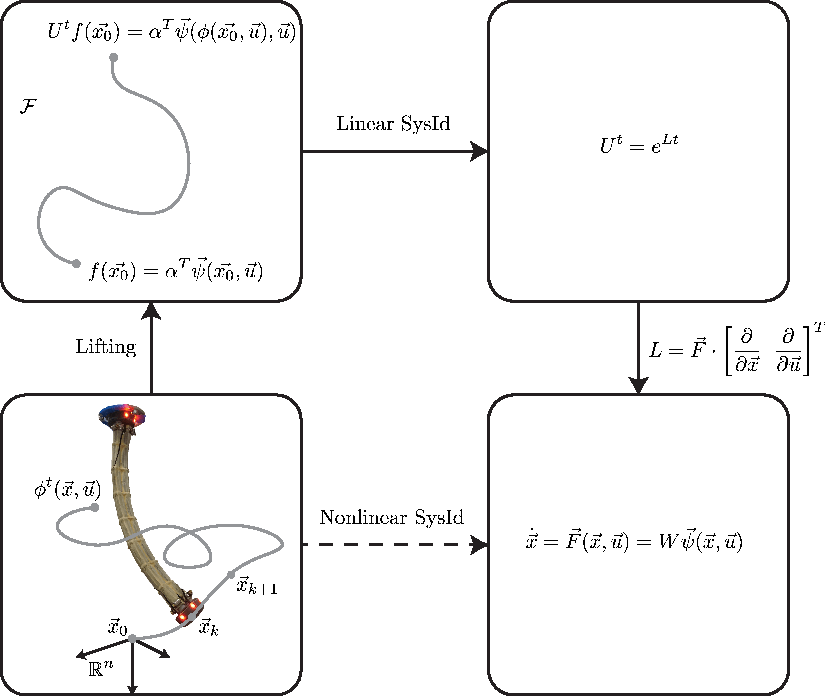
\includegraphics[width=\linewidth]{figures/overviewDiagram_rough.pdf}
    \caption{Caption: Overview of sysid method}
    \label{fig:overview}
\end{figure}

%% Soft robots are particularly well suited for system identification
White box models \Ram{what is a white box model?} for soft robots based on first principles are typically insufficient or too complex to be used for control, for the reasons stated above \Ram{This is again a fairly sharp transition and is lacking in references.}. 
However, by virtue of their soft bodies it is often possible to safely command arbitrary control inputs without risk of damaging a soft robot or nearby human operators.
Thus, soft robots are amenable to data collection over their entire operation range, making them particularly well suited for data-driven system identification techniques.
% Since a white-box model based on first principles, e.g. a model for a physical process from the Newton equations, are typically unavailable or too complicated to be used in control due to the complex nature of soft robots, (grey and black box models built via) system identification are needed.
%% Linear system identification is trivial
For linear systems, system identification trivially \Ram{don't use words like trivial or intuitive. Its a mean thing to say to a reader who does not understand.} consists of fitting a linear model to observed data via linear regression \Ram{reference?} \Ram{you probably also want to say that linear system id is somehow not applicable to soft robot and cite a reference.}.
%% Nonlinear system identification is hard
For nonlinear systems, identifying a model is much more difficult since it consists of solving a nonlinear non-convex optimization problem, for which global convergence is not guaranteed \Ram{reference?}.

%% Neural network has successfully been applied to soft robot
Despite its challenges, nonlinear system identification has been demonstrated successfully on soft robots in the past \Ram{This is an awkward sentence. What does it mean to demonstrate successfully? }.
In \cite{gillespie2018learning} a Deep Neural Network (DNN) was used to model the behavior of a 1 DOF pneumatic soft robot arm.
The resulting MPC \Ram{spell out the first time} controller with the neural network model acting as its predictor performed comparably to an MPC controller with a much more complicated white box model \Ram{make sure you define white box at some point}.
While in this case the neural network model was effective, a weakness of neural network models in general is the extent to which the training process is heuristic in nature.
A neural network model depends on the specific training parameters chosen (e.g. number of hidden layers, number of nodes per layer, activation function, termination condition), and training may result in a sub-optimal neural network model for a given set of data.
\Ram{be more explicit about the potential shortcomings...}

%% Koopman let's us do linear sysid (trivial) on a nonlinear system
A more reliable system identification approach utilizes operator-theoretic techniques to perform linear system identification of nonlinear systems \Ram{what does more reliable mean?}.
This approach relies on the idea of lifting nonlinear dynamical systems to an infinite dimensional space, where those systems have a linear representation.
\Ram{maybe these next few sentences are too much detail for now since that is something you are going to present later on...maybe just highlight its strengths? You may want to reference the figure you have developed as well.}
The Koopman Operator is a linear operator that describes the flow of observable functions of state along trajectories of the system.
By exploiting the lifting obtained through the Koopman Operator, it is possible to describe the dynamic behavior of the system by identifying a linear operator in the space of observables instead of identifying a nonlinear systems in the state space.
This linear operator is identified via linear regression, so it does not suffer from the indeterminacy of other nonlinear system identification methods.
% Since the Koopman operator is defined on an infinite-dimensional vector space, in practice it must be projected onto a finite basis of observable functions.
% However, with a suitably large finite dimensional approximation, we demonstrate that we can capture the true nonlinear system dynamics of a soft robot arm more accurately and more reliably than several other nonlinear system identification methods.

\Ram{I think you need a sentence here listing out the contributions of this paper....}
In this paper we apply the Koopman based system identification method described in \cite{mauroy2016linear} and \cite{mauroy2017koopman} to create a dynamic model of a soft robot arm and demonstrate that it captures the system's true dynamic behavior better than the models generated by several other state-of-the-art nonlinear system identification methods including a neural network model, a nonlinear auto-regressive moving average model with exogenous inputs (NARMAX model), a nonlinear Hammerstein-Wiener model, and a state space model.

%% Why is this contribution significant?: Could enable real-time sysid/control, MPC, 
To the author's knowledge, this technique has never before been used to identify the dynamic model of a real system, much less a soft robot.
We believe that this system identification method applied to soft robots will enable the rapid development of new and effective control strategies by making accurate nonlinear dynamic models easier to construct.
% We believe that the models generated are accurate enough to be useful in control applications such as predictors in MPC controllers.
% Due to its numerical simplicity, this method also has the potential to be incorporated into real-time simultaneous sysid/control applications.

%% Outline of the rest of this paper
The rest of this paper is organized as follows:
In Section \ref{sec:theory} we formally introduce the Koopman Operator and describe the system identification method. 
In Section \ref{sec:experiment} we describe the soft robot and experimental procedure used for collecting input-output data of the system.
In Section \ref{sec:results} we summarize the results of applying various nonlinear system identification techniques to the collected data and compare the performances of the models generated. Concluding remarks and perspectives are provided in section \ref{sec:conclusion}.
